\documentclass{article} %article 文档
\usepackage{ctex}  %使用宏包(为了能够显示汉字)
\usepackage[hidelinks]{hyperref}
\usepackage{color}
\usepackage{amsmath}

%2个图片包
\usepackage{graphicx}
\usepackage{epstopdf}

\title{高等数学笔记}  %文章标题
\author{}   %作者的名称
\date{}       %日期
% 设置页面的环境,a4纸张大小,左右上下边距信息
\usepackage[a4paper,left=10mm,right=10mm,top=15mm,bottom=15mm]{geometry}  
\begin{document} %正文部分
\maketitle          %添加这一句才能够显示标题等信息

%目录页
\tableofcontents
\thispagestyle{empty}
\clearpage
\setcounter{page}{1}





%正文
\section{多元函数微分法及其应用}
\subsection{多元函数的基本概念}
\subsubsection{平面点集 *n维空间}
\begin{enumerate}
    \item {
        \textbf{平面点集}
        \begin{description}
            \item[内点] {在函数的图形内}
            \item[外点] {在函数的图形外}
            \item[边界点] {在函数的图形边界上}
            \item[聚点] {图形区域内的点,不包括离群的离散点}
            \item[开集] {不能取到边界点的点集}
            \item[闭集] {能取到边界点的点集}
            \item[区域] {集合内任意两点能通过连续折线段连接的点集}
            \item[开区域]{能取到边界点的区域}
            \item[闭区域]{不能取到边界点的区域} 
        \end{description}

        对区域 $D$ , 若存在正数 $K$ , 使一切点 $P\in D$ 与某定点 $A$ 的距离 $|AP|\leq K$ ,则称 $D$ 为\textbf{有界域} , 否则称为\textbf{无界域}
    }
    
    \item {
        \textbf{平面点集}\\
        有n个坐标。
    }
\end{enumerate}

\subsubsection{多元函数的概念}
\begin{itemize}
    \item {
        \textbf{多元函数} \hspace{2mm}有多个自变量的函数$f(x_1,x_2...)$
    }

    \item {
        \textbf{自然定义域} \hspace{2mm}使函数$f(x_1,x_2...)$有意义的点集
    }

    \item {
        \textbf{函数的图形} \hspace{2mm}自然定义域构成的图形
    }
\end{itemize}

\textcolor{red}{注:一元函数的性质对多元函数也同样适用(包括:介值定理、有界性与最大最小值定理,一致连续性定理)}

\subsubsection{多元函数的极限}
\textbf{定义通俗点:}\par
\hspace{10mm}当从任意方向像点$(x,y)$逼近时,对应的函数值趋近于同一个数,则极限存在,称作\textcolor{red}{二重极限}\par
\hspace{10mm}记作$\displaystyle \lim_{(x,y)\to(x_0,y_0)}f(x,y)=A$或$\displaystyle \lim_{P\to P_0}f(P)=A$\par
\textcolor{red}{注:一元函数的极限运算法则对多元函数也同样适用}

\subsubsection{多元函数的连续性}
\begin{itemize}
    \item 若$\displaystyle \lim_{(x,y)\to(x_0,y_0)}f(x,y)=f(x_0,y_0)$,则函数在$P_0(x_0,y_0)$处连续。
    \item 若函数在$D$上有定义且处处连续,则称函数为\textcolor{red}{$D$上的连续函数}
    \item 若函数在$P_0(x_0,y_0)$处不连续,则称$P_0$为函数的间断点
\end{itemize}

\textcolor{red}{注:一切多元函初等函数在定义区域内是连续的}

\subsection{偏导数}
\subsubsection{偏导数的定义及其计算方法}
\textbf{定义通俗点:}\par
\hspace{10mm}将其他自变量$y...$固定(看做常量),只对其中一个自变量$x$求导\par
\vspace{5mm} 
$f(x,y)$在$(x_0,y_0)$处对$x$的偏导数为$\displaystyle \lim_{\Delta x\to 0}{f(x_0+\Delta x,y_0)-f(x_0,y_0) \over \Delta x}$\par
记作
$\displaystyle\left.\frac{\partial f}{\partial x}\right|_{x=x_0,y=y_0}$,
$\displaystyle\left.\frac{\partial z}{\partial x}\right|_{x=x_0,y=y_0}$,
$\displaystyle\left.z_x\right|_{x=x_0,y=y_0}$,
$\displaystyle f_x(x_0,y_0)$\par
\vspace{5mm} 
\begin{tabular}{rl}
    一般将函数$f(x,y)$ & 对$x$的偏导记作
    $\displaystyle \frac{\partial f}{\partial x}$,
    $\displaystyle \frac{\partial z}{\partial x}$,
    $\displaystyle z_x$,
    $\displaystyle f_x(x,y)$\vspace{3mm}\\
    
    & 对$y$的偏导记作
    $\displaystyle \frac{\partial f}{\partial y}$,
    $\displaystyle \frac{\partial z}{\partial y}$,
    $\displaystyle z_y$,
    $\displaystyle f_y(x,y)$
\end{tabular}\par
\vspace{2mm}
\textcolor{red}{注:偏导符号是一个整体,不能看做$\partial z$与$\partial x$相除}\par
\vspace{3mm}
\textcolor{red}{多元函数同理}\par
\vspace{3mm}
\textbf{偏导数$\displaystyle f_x(x_0,y_0)$的几何意义:}\par
\hspace{10mm}曲面被$x=x_0$所截得的曲线的导数


\vspace{5mm}
\textcolor{red}{注:二元函数在某点如果偏导数都存在,但在该点不一定连续。}


\subsubsection{高阶偏导数}
\textbf{通俗点:}\par
\hspace{10mm}若偏导的偏导存在,对偏导再求一次偏导,即二阶偏导。一直循环下去\par
\hspace{10mm}注:在求高阶偏导时可以换个维度求\par
形如:
$$
\begin{array}{lcl}
    \displaystyle \frac{\partial}{\partial x}\left(\frac{\partial z}{\partial x}\right)=\frac{\partial^2 z}{\partial x^2}=f_{xx}(x,y) &
    &
    \displaystyle \frac{\partial}{\partial y}\left(\frac{\partial z}{\partial x}\right)=\frac{\partial^2 z}{\partial x \partial y}=f_{xy}(x,y) \vspace{2mm}\\
    \displaystyle \frac{\partial}{\partial y}\left(\frac{\partial z}{\partial y}\right)=\frac{\partial^2 z}{\partial y^2}=f_{yy}(x,y) &
    &
    \displaystyle \frac{\partial}{\partial x}\left(\frac{\partial z}{\partial y}\right)=\frac{\partial^2 z}{\partial y \partial x}=f_{yx}(x,y) \\
\end{array}
$$\par
后列称为\textcolor{red}{混合偏导数}\par
\vspace{3mm}
\textbf{定理:}\par
\hspace{10mm}若$\displaystyle\frac{\partial^2 z}{\partial y \partial x}$及$\displaystyle\frac{\partial^2 z}{\partial x \partial y}$在区域$D$内连续,那么该区内这两个二阶混合偏导数必定相等。\par
\textbf{通俗点:}二阶混合偏导数在连续的条件下与求导的次序无关。\par
\vspace{5mm}
\textbf{*拉普拉斯(Laplace)方程:}\par

\hspace{20mm}1.$z=\ln{\sqrt{x^2+y^2}}$满足方程$\displaystyle\frac{\partial^2 z}{\partial x^2}+\frac{\partial^2 z}{\partial y^2}=0$\par
\hspace{3mm}

\hspace{20mm}2.$\displaystyle u={1\over\sqrt{x^2+y^2+z^2}}$满足方程$\displaystyle\frac{\partial^2 u}{\partial x^2}+\frac{\partial^2 u}{\partial y^2}+\frac{\partial^2 u}{\partial z^2}=0$\par


\subsection{全微分}
\subsubsection{全微分的定义}
$dz=A\Delta x+B\Delta y$\par
\hspace{3mm}

\textbf{必要条件:}\par
\hspace{10mm}若函数$z=f(x,y)$在$(x,y)$可微分,那么该函数在$(x,y)$的偏导数$\displaystyle \frac{\partial z}{\partial x}$与$\displaystyle \frac{\partial z}{\partial x}$必定\textcolor{red}{存在},\par
\hspace{10mm}且$z=f(x,y)$的全微分为$dz=\displaystyle \frac{\partial z}{\partial x}\Delta x+\displaystyle \frac{\partial z}{\partial y}\Delta y$

\textbf{充分条件:}\par
\hspace{10mm}若函数$z=f(x,y)$在$(x,y)$的偏导数$\displaystyle \frac{\partial z}{\partial x}$、$\displaystyle \frac{\partial z}{\partial y}$在$(x,y)$\textcolor{red}{连续},那么函数在该点可微分

\begin{figure}[htbp]
    \centering
    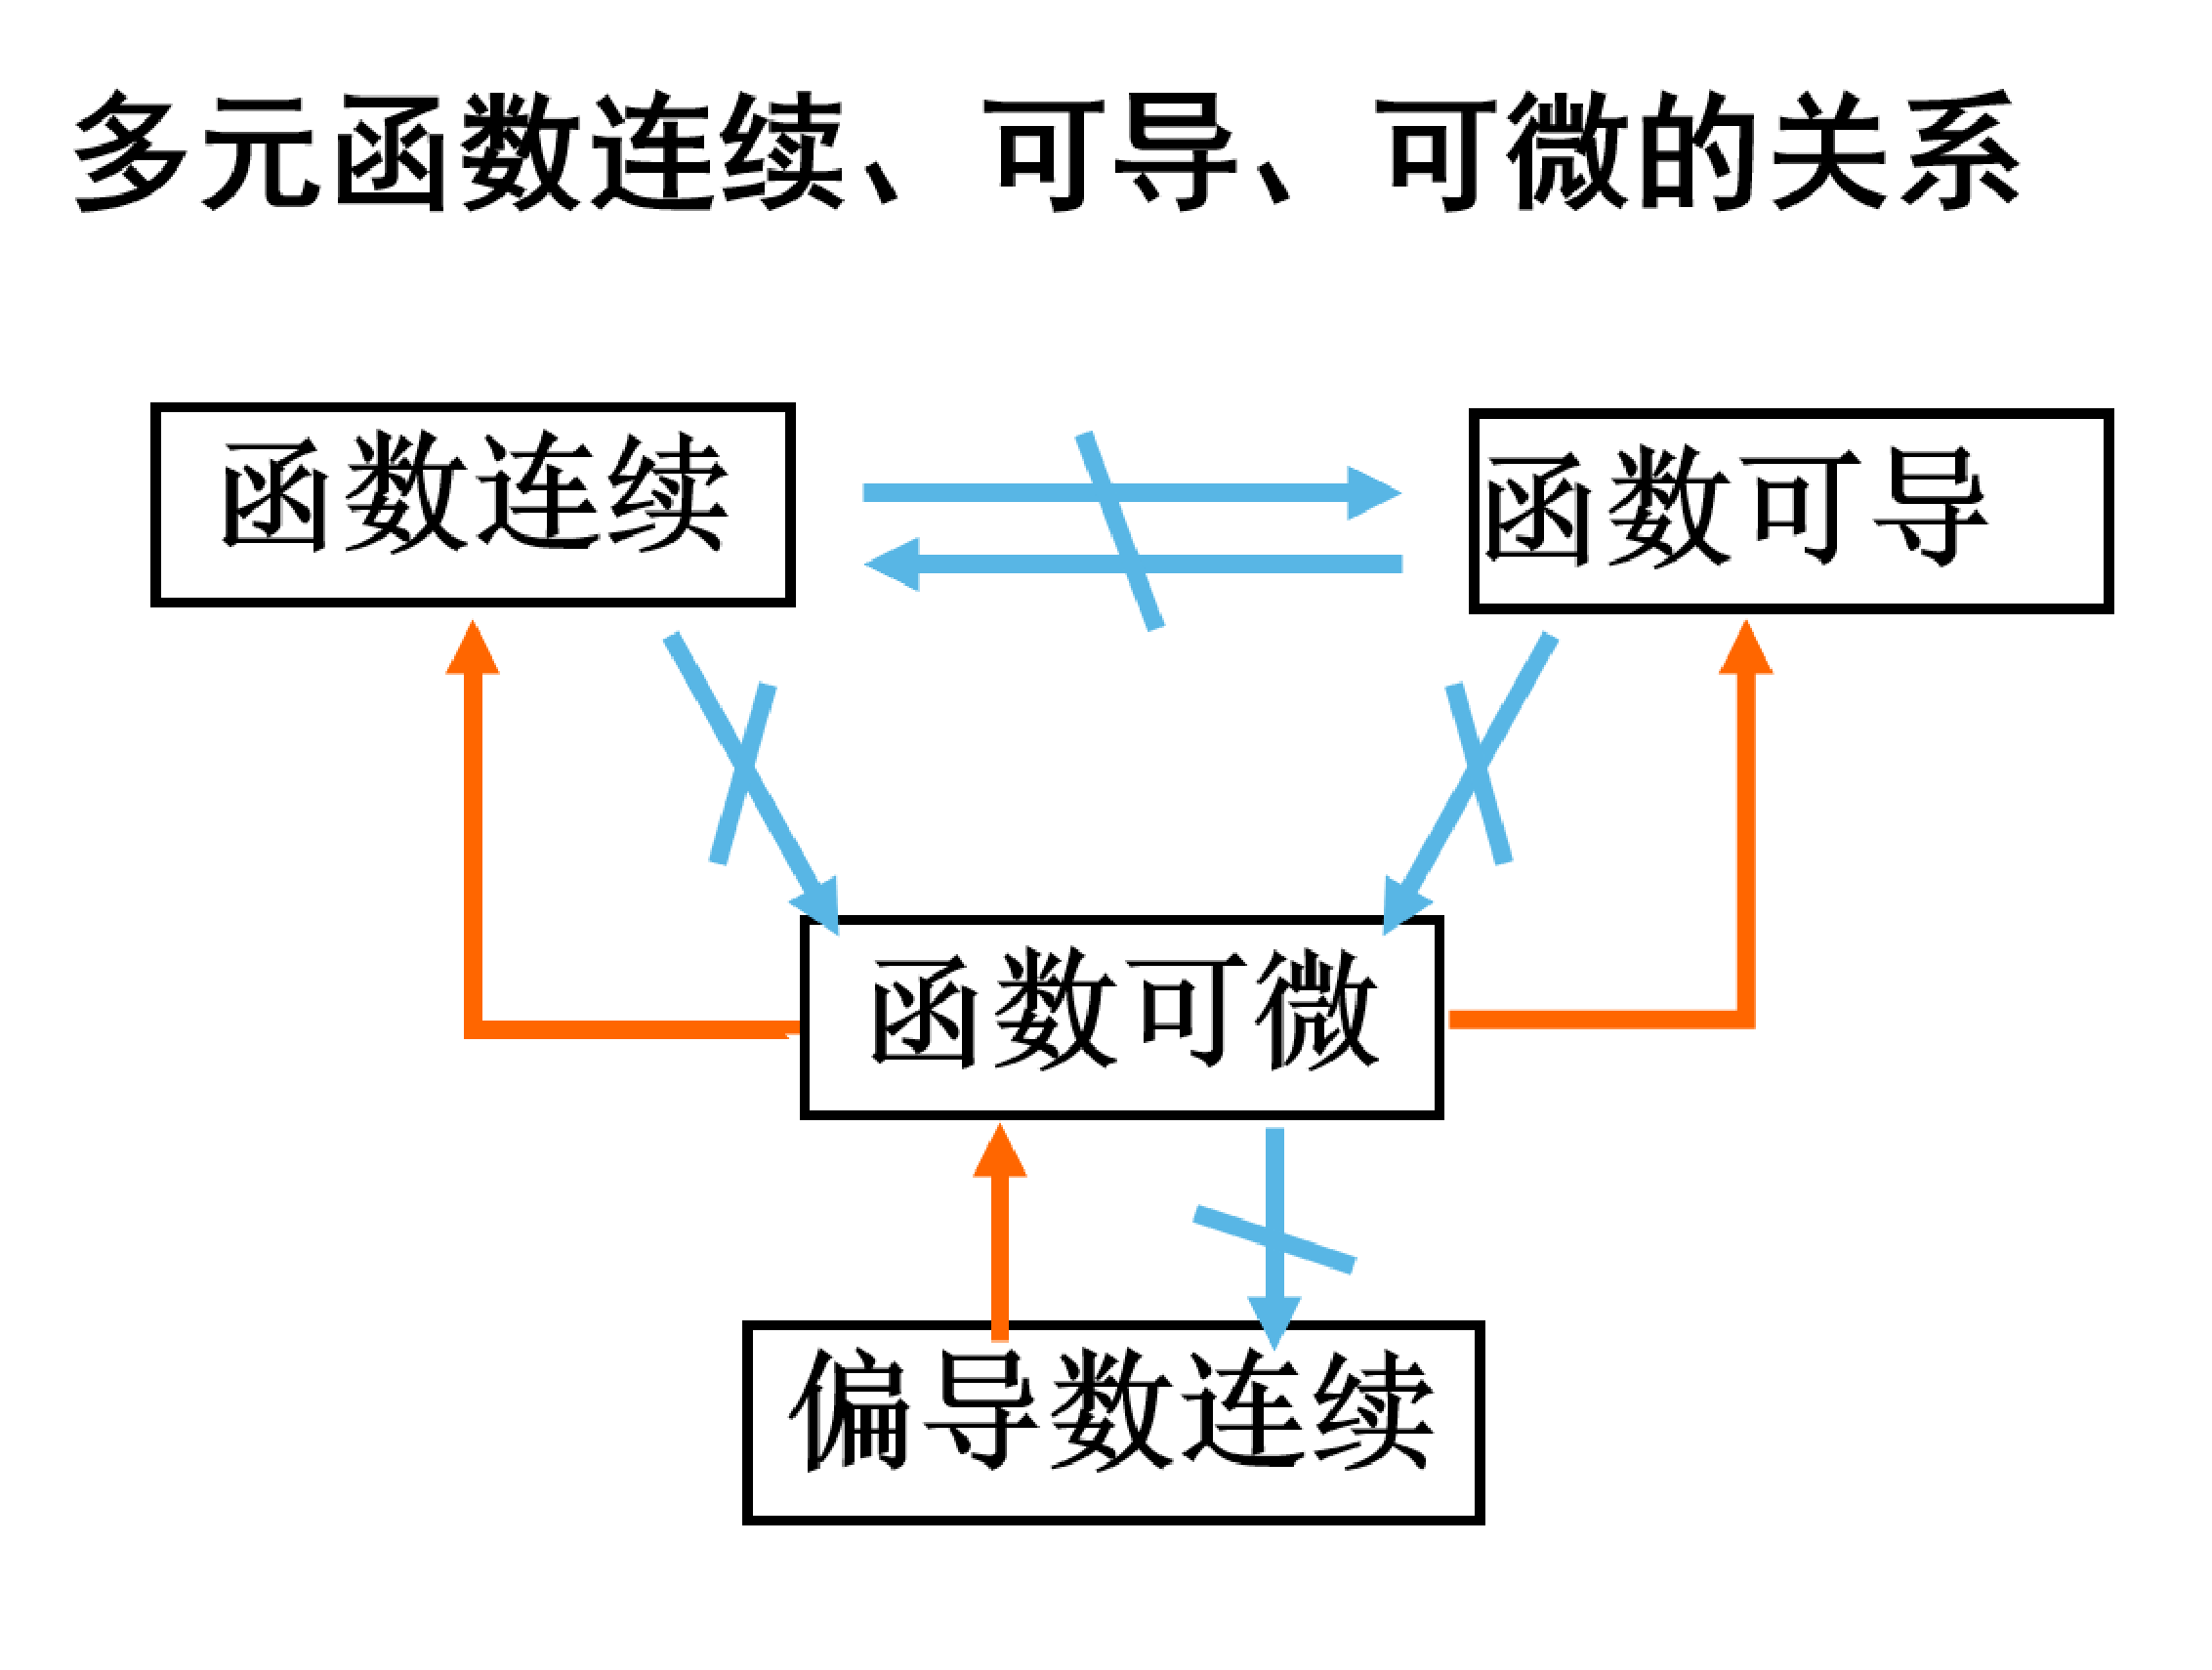
\includegraphics[scale=0.15]{p9-1.eps}
    % \caption{figure title}
    \label{figure}
\end{figure}
    
\subsubsection{*全微分在近似计算中的应用}


\subsection{多元复合函数的求导法则}
% \clearpage
\subsubsection{一元函数与多元函数复合}
已知函数$u=g(t),v=h(t)$ 函数$z=f[g(t),h(t)]$\par
则$\displaystyle dz=\frac{\partial z}{\partial u}\frac{du}{dt}+\frac{\partial z}{\partial v}\frac{dv}{dt}$

\subsubsection{多元函数与多元函数复合}
已知函数$u=g(x,y),v=h(x,y)$ 函数$z=f(u,v)$\par
\vspace{1mm}

则$
\begin{array}{ll}
    \displaystyle \frac{\partial z}{\partial x}=\frac{\partial z}{\partial u}\frac{\partial u}{\partial x}+\frac{\partial z}{\partial v}\frac{\partial v}{\partial x} \vspace{2mm}\\
    \displaystyle \frac{\partial z}{\partial y}=\frac{\partial z}{\partial u}\frac{\partial u}{\partial y}+\frac{\partial z}{\partial v}\frac{\partial v}{\partial y}
\end{array}$

\subsubsection{其他情形}
\begin{enumerate}
    \item 与一元和多元函数复合\\已知函数$u=g(x,y),v=h(y)$ 函数$z=f(u,v)$\par
        \vspace{1mm}

        则$
        \begin{array}{ll}
            \displaystyle \frac{\partial z}{\partial x}=\frac{\partial z}{\partial u}\frac{\partial u}{\partial x} \vspace{2mm}\\
            \displaystyle \frac{\partial z}{\partial y}=\frac{\partial z}{\partial u}\frac{\partial u}{\partial y}+\frac{\partial z}{\partial v}\frac{d v}{d y}
        \end{array}$
    \item 有些中间变量还是复合函数的自变量\\
        如$z=f[g(x,y),x,y]$,可看做$v=x,w=y$的特殊形式\\
        则$\begin{array}{cc}
            \displaystyle\frac{\partial v}{\partial x}=1 & \displaystyle\frac{\partial w}{\partial x}=0 \vspace{2mm}\\
            \displaystyle\frac{\partial v}{\partial y}=0 & \displaystyle\frac{\partial w}{\partial y}=1\\
        \end{array}$\\
        \vspace{2mm}

        得到$\begin{array}{l}
            \displaystyle\frac{\partial z}{\partial x}=\frac{\partial f}{\partial u}\frac{\partial u}{\partial x}+\frac{\partial f}{\partial x}\vspace{2mm}\\
            \displaystyle\frac{\partial z}{\partial y}=\frac{\partial f}{\partial u}\frac{\partial u}{\partial y}+\frac{\partial f}{\partial y}\\
        \end{array}$

        \textcolor{red}{
        \begin{tabular}{ll}
            注意: & $\frac{\partial z}{\partial x}$把$f[g(x,y),x,y]$中的$y$看做不变\\
                     & $\frac{\partial f}{\partial x}$把$f[u,x,y]$中的$u,y$看做不变\\
        \end{tabular}
        }
    \item 全微分形式不变性 \vspace{1mm}\\
        $z=f(u,v)$的全微分为
        $\displaystyle dz=\frac{\partial z}{\partial u}du+\frac{\partial z}{\partial v}dv$\\
        若$u=g(x,y),v=h(x,y)$\\
        则$\displaystyle dz=\frac{\partial z}{\partial x}dx+\frac{\partial z}{\partial y}dy$\\
        \vspace{1mm}

        可见,无论$u,v$是中间变量,还是自变量,函数$z=f(u,v)$的全微分形式都一样\\这个性质叫做\textcolor{red}{全微分的形式不变性}。
\end{enumerate}

% \vspace{10mm}
\subsubsection{求复合函数微分的小技巧}
在求复合函数的微分时,可以先画出复合关系的树状图,然后再对应每条路径按最终变量分类别求和即可。\par
如下图所示:

\begin{figure}[htbp]
    \centering
    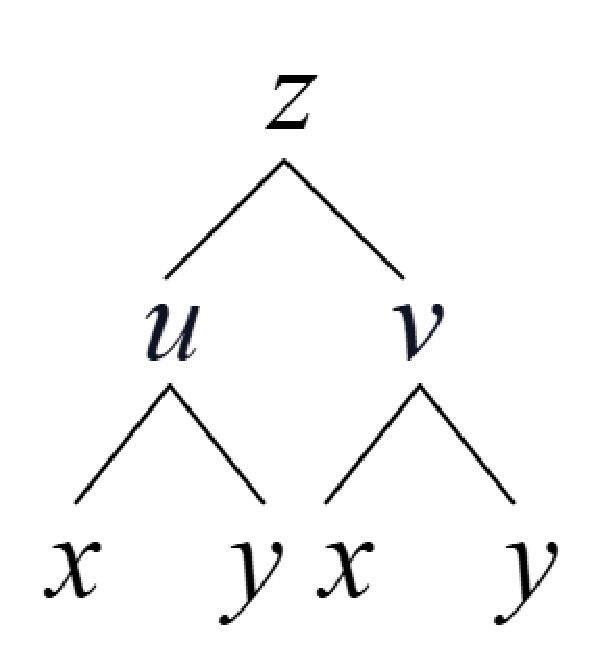
\includegraphics[scale=0.3]{p9-2.eps}
    % \caption{figure title}
    \label{figure}
\end{figure}


\subsection{隐函数的求导公式}
\subsubsection{一个方程的情形}
\begin{itemize}
    \item $F(x,y)=0$\vspace{1mm}\\
        $\displaystyle
        \frac{dy}{dx}=-\frac{F_x}{F_y}
        $\vspace{1mm}\\
        \textcolor{red}{注意方程右边是倒过来的,对x的偏微分在上,对y的偏微分在下}\\
        % \vspace{1mm}
        可由$F(x,f(x))=0 $得到\vspace{1mm}\\
        $\displaystyle\Rightarrow \frac{\partial F}{\partial x}+\frac{\partial F}{\partial y}\frac{dy}{dx}=0\\
        \Rightarrow\frac{dy}{dx}=-\frac{F_x}{F_y}$
    \item $F(x,y,z)=0$\vspace{1mm}\\
        $\displaystyle
        \frac{\partial z}{\partial x}=-\frac{F_x}{F_z},
        \frac{\partial z}{\partial y}=-\frac{F_y}{F_z}
        $%\vspace{1mm}\\
        \\
        可由$F(x,y,f(x,y))=0$得到\\
        $\displaystyle\Rightarrow F_x+F_z\frac{\partial z}{\partial x}=0,F_y+F_z\frac{\partial z}{\partial y}=0\\
        \Rightarrow
        \frac{\partial z}{\partial x}=-\frac{F_x}{F_z},
        \frac{\partial z}{\partial y}=-\frac{F_y}{F_z}
        $
\end{itemize}


\subsubsection{方程组的情形}
对方程组$\left\{
    \begin{array}{ll}
        F(x,y,u,v)=0\\
        G(x,y,u,v)=0
    \end{array}
\right.$\par
雅可比式$\displaystyle
J=\frac{\partial (F,G)}{\partial (u,v)}=\left|
\begin{array}{cc}
    \frac{\partial F}{\partial u} & \frac{\partial F}{\partial v} \\
    \frac{\partial G}{\partial u} & \frac{\partial G}{\partial v} \\
\end{array}
\right|
$

$$
\frac{\partial u}{\partial x}=-\frac{1}{J}\frac{\partial(F,G)}{\partial(x,v)}=
-{\left|\begin{array}{cc}
    F_x & F_v\\
    G_x & G_v\\
\end{array}\right|
\over
\left|\begin{array}{cc}
    F_u & F_v\\
    G_u & G_v\\
\end{array}\right|
}
\hspace{10mm}
\frac{\partial v}{\partial x}=-\frac{1}{J}\frac{\partial(F,G)}{\partial(u,x)}=
-{\left|\begin{array}{cc}
    F_u & F_x\\
    G_u & G_x\\
\end{array}\right|
\over
\left|\begin{array}{cc}
    F_u & F_v\\
    G_u & G_v\\
\end{array}\right|
}
$$
$$
\frac{\partial u}{\partial y}=-\frac{1}{J}\frac{\partial(F,G)}{\partial(y,v)}=
-{\left|\begin{array}{cc}
    F_y & F_v\\
    G_y & G_v\\
\end{array}\right|
\over
\left|\begin{array}{cc}
    F_u & F_v\\
    G_u & G_v\\
\end{array}\right|
}
\hspace{10mm}
\frac{\partial v}{\partial y}=-\frac{1}{J}\frac{\partial(F,G)}{\partial(u,y)}=
-{\left|\begin{array}{cc}
    F_u & F_y\\
    G_u & G_y\\
\end{array}\right|
\over
\left|\begin{array}{cc}
    F_u & F_v\\
    G_u & G_v\\
\end{array}\right|
}
$$

可由$F[x,y,u(x,y),v(x,y)]=0,G[x,y,u(x,y),v(x,y)]=0$得到\par
对$x$求导\par
$\displaystyle\Rightarrow 
    \left\{\begin{array}{l}
        \displaystyle F_x+F_u\frac{\partial u}{\partial x}+F_v\frac{\partial v}{\partial x}=0\vspace{1mm}\\
        \displaystyle G_x+G_u\frac{\partial u}{\partial x}+G_v\frac{\partial v}{\partial x}=0\\
    \end{array}\right.$\vspace{2mm}\par
通过解非齐次线性方程组得到\par
$\displaystyle
\Rightarrow
\frac{\partial u}{\partial x}=-\frac{1}{J}\frac{\partial (F,G)}{\partial (x,v)},
\frac{\partial v}{\partial x}=-\frac{1}{J}\frac{\partial (F,G)}{\partial (u,x)}
$
\par
对$y$求导同理

\subsection{多元函数微分学的几何应用}
\subsubsection{一元向量值函数及其导数}
$f(t)=f_1(t)\vec{i}+f_2(t)\vec{j}+f_3(t)\vec{k}$\par
$f'(t)=f'_1(t)\vec{i}+f'_2(t)\vec{j}+f'_3(t)\vec{k}$表示曲线的切向方向\par
\vspace{3mm}
一些运算法则
\begin{enumerate}
    \item $\displaystyle\frac{d}{dt}\vec{C}=\vec{0}$
    \item $\displaystyle\frac{d}{dt}[c\vec{u}(t)]=c\vec{u}'(t)$
    \item $\displaystyle\frac{d}{dt}[\vec{u}(t)+\vec{v}(t)]=\vec{u}'(t)+\vec{v}'(t)$
    \item $\displaystyle\frac{d}{dt}[\phi(t)\vec{u}(t)]=\phi'(t)\vec{u}(t)+\phi(t)\vec{u}'(t)$
    \item $\displaystyle\frac{d}{dt}[\vec{u}(t)\cdot\vec{v}(t)]=\vec{u}'(t)\cdot\vec{v}(t)+\vec{u}(t)\cdot\vec{v}'(t)$
    \item $\displaystyle\frac{d}{dt}[\vec{u}(t)\times\vec{v}(t)]=\vec{u}'(t)\times\vec{v}(t)+\vec{u}(t)\times\vec{v}'(t)$
    \item $\displaystyle\frac{d}{dt}\vec{u}[\phi(t)]=\phi'(t)\vec{u}'[\phi(t)]$
\end{enumerate}

\subsubsection{空间曲线的切线与法平面}
\begin{enumerate}
    \item 曲线
        $\left\{ \begin{array}{l}
            x=f(t)\\y=g(t)\\z=h(t)
        \end{array}\right.$\par
        切线方程\textcolor{red}{$\displaystyle\frac{x-x_0}{f'(t_0)}=\frac{y-y_0}{g'(t_0)}=\frac{z-z_0}{h'(t_0)}$}\vspace{2mm}\par
        法平面方程\textcolor{red}{$f'(t_0)(x-x_0)+g'(t_0)(y-y_0)+h'(t_0)(z-z_0)=0$}
    \item 曲线
        $\left\{ \begin{array}{l}
            x=x\\y=f(x)\\z=g(x)
        \end{array}\right.$\par
        切线方程\textcolor{red}{$\displaystyle\frac{x-x_0}{1}=\frac{y-y_0}{f'(x_0)}=\frac{z-z_0}{g'(x_0)}$}\vspace{2mm}\par
        法平面方程\textcolor{red}{$(x-x_0)+f'(x_0)(y-y_0)+g'(x_0)(z-z_0)=0$}
    \item 曲线
        $\left\{ \begin{array}{l}
            F(x,y,z)=0\\G(x,y,z)=0
        \end{array}\right.$\par
        切线方程\textcolor{red}{
            $\displaystyle
                \frac{x-x_0}{\left|\begin{array}{cc}F_y&F_z\\G_y&G_z\end{array}\right|_M}
                =
                \frac{y-y_0}{\left|\begin{array}{cc}F_z&F_x\\G_z&G_x\end{array}\right|_M}
                =
                \frac{z-z_0}{\left|\begin{array}{cc}F_x&F_y\\G_x&G_y\end{array}\right|_M}$}\vspace{2mm}\par
        法平面方程\textcolor{red}{
            $\displaystyle
            \left|\begin{array}{cc}F_y&F_z\\G_y&G_z\end{array}\right|_M(x-x_0)+
            \left|\begin{array}{cc}F_z&F_x\\G_z&G_x\end{array}\right|_M(y-y_0)+
            \left|\begin{array}{cc}F_x&F_y\\G_x&G_y\end{array}\right|_M(z-z_0)=0$}\par
        具体推导过程参见下册书本$P98$
\end{enumerate}

\subsubsection{曲面的切平面与法线}
\begin{enumerate}
    \item 曲面$F(x,y,z)=0$\par
        切面方程\textcolor{red}{$F_x(x_0,y_0,z_0)(x-x_0)+F_y(x_0,y_0,z_0)(y-y_0)+F_z(x_0,y_0,z_0)(z-z_0)=0$}\vspace{2mm}\par
        法向量\textcolor{red}{$\vec{n}=(F_x(x_0,y_0,z_0),F_y(x_0,y_0,z_0),F_z(x_0,y_0,z_0))$}\vspace{2mm}\par
        法线方程\textcolor{red}{$\displaystyle
            \frac{x-x_0}{F_x(x_0,y_0,z_0)}=
            \frac{y-y_0}{F_y(x_0,y_0,z_0)}=
            \frac{z-z_0}{F_z(x_0,y_0,z_0)}
            $}
    \item 曲面$z=f(x,y)$\par
        切面方程\textcolor{red}{$f_x(x_0,y_0)(x-x_0)+f_y(x_0,y_0)(y-y_0)-(z-z_0)=0$}\vspace{2mm}\par
        法向量\textcolor{red}{$\vec{n}=(f_x(x_0,y_0),f_y(x_0,y_0),-1)$}\vspace{2mm}\par
        法线方程\textcolor{red}{$\displaystyle
            \frac{x-x_0}{f_x(x_0,y_0)}=
            \frac{y-y_0}{f_y(x_0,y_0)}=
            \frac{z-z_0}{-1}
        $}\\
        法向量的方向余弦\textcolor{red}{$\displaystyle
            \cos\alpha={-f_x\over\sqrt{1+f_x^2+f_y^2}},
            \cos\beta={-f_y\over\sqrt{1+f_x^2+f_y^2}},
            \cos\gamma={1\over\sqrt{1+f_x^2+f_y^2}}$}
\end{enumerate}

\subsection{方向导数与梯度}
\subsubsection{方向导数}
\begin{enumerate}
    \item 二元函数$f(x,y)$\\
        $\displaystyle 
        \left.\frac{\partial f}{\partial l}\right|_{(x_0,y_0)}
        =f_x(x_0,y_0)\cos\alpha+f_y(x_0,y_0)\cos\beta$

    \item 三元函数$f(x,y,z)$\\
        $\displaystyle 
        \left.\frac{\partial f}{\partial l}\right|_{(x_0,y_0,z_0)}
        =f_x(x_0,y_0,z_0)\cos\alpha+f_y(x_0,y_0,z_0)\cos\beta+f_z(x_0,y_0,z_0)\cos\gamma$
\end{enumerate}

\begin{tabular}{ll}
    \textcolor{red}{\textbf{注:}} & 偏导数存在 \textcolor{red}{\textbf{可以推出}} 方向导数存在\\
    & 方向导数存在 \textcolor{red}{\textbf{不能推出}} 偏导数存在
\end{tabular}


\subsubsection{梯度}
$\nabla f(x_0,y_0)=f_x(x_0,y_0)\vec{i}+f_y(x_0,y_0)\vec{j}$\vspace{5mm}\par
设$\vec{e}_l$为函数在$l$方向的单位向量\vspace{1mm}\par
则$\displaystyle\left.\frac{\partial f}{\partial l}\right|_{(x_0,y_0)}=\nabla f(x_0,y_0)\cdot\vec{e}$\vspace{1mm}\par
梯度与$l$方向的夹角$\theta=\left\langle \nabla f(x_0,y_0),\vec{e}_l \right\rangle  $
\begin{enumerate}
    \item 当$\theta=0$时,$f(x,y)$增加最快。\\
        函数在这个方向的方向导数达到最大值,\\
        这个最大值也就是梯度$\nabla f(x_0,y_0)$的模,即$\displaystyle |\nabla f(x_0,y_0)|=\left.\frac{\partial f}{\partial l}\right|_{(x_0,y_0)}$
    \item 当$\theta=\pi$时,$f(x,y)$减少最快。\\
        函数在这个方向的方向导数达到最小值
    \item 当$\theta=\frac{\pi}{2}$时,$f(x,y)$变化率为0。\\
    
\end{enumerate}

三维的梯度同理

\subsection{多元函数的极值与求法}
\subsubsection{多元函数的极值及最大值最小值}
有极值的\textbf{必要条件}\par
\hspace{5mm}有极值$\Rightarrow \left\{\begin{array}{l}f_x(x_0,y_0)=0\\f_y(x_0,y_0)=0\end{array}\right.$\par
有极值的\textbf{充分条件}\par
\hspace{5mm}令$f_{xx}(x_0,y_0)=A,f_{xy}(x_0,y_0)=B,f_{yy}(x_0,y_0)=C$\par
\hspace{5mm}1.$AC-B^2>0$时有极值,$A<0$时为极大值,$A>0$时为极小值\par
\hspace{5mm}2.$AC-B^2<0$时无极值\par
\hspace{5mm}3.$AC-B^2=0$时可能有极值,也可能没有极值,需另外讨论\par

\subsubsection{条件极值、拉格朗日乘数法}
\textbf{拉格朗日乘数法}\par
\hspace{5mm}要找$z=f(x,y)$在附加条件$\phi(x,y)=0$下的可能极值点\par
\hspace{5mm}可以先作拉格朗日函数$L(x,y)=f(x,y)+\lambda\phi(x,y)$\par
\hspace{5mm}然后求其对$x,y$的偏导数,与条件联立得到\par
\hspace{5mm}$\left\{\begin{array}{ll}
        f_x(x,y)+\lambda\phi_x(x,y)=0\\
        f_y(x,y)+\lambda\phi_y(x,y)=0\\
        \phi(x,y)=0
    \end{array}\right.$\par
\hspace{5mm}由这组方程得到的(x,y)就是$f(x,y)$在附加条件$\phi(x,y)$下的可能极值点

\subsection{*二元函数的泰勒公式}
\subsubsection{二元函数的泰勒公式}
\subsubsection{极值充分条件的证明}

\subsection{*最小二乘法}






\end{document}